\documentclass{article}
\usepackage[T1]{fontenc}
\usepackage{lmodern}
\usepackage{graphicx}
\usepackage{amsmath,amssymb}
\usepackage[a4paper,margin=2cm]{geometry}
\usepackage[absolute,overlay]{textpos}
\setlength{\TPHorizModule}{1mm}
\setlength{\TPVertModule}{1mm}
\usepackage[indonesian]{babel}
\usepackage{hyperref}
\setlength{\emergencystretch}{2em}
% unit: Halaman 88

\begin{document}

% === Halaman 88 (llm) ===

% (tidak ada teks dari model)

% deskripsi: Screenshot kode program Python untuk fungsi EmbeddingPesan yang mengimplementasikan teknik steganografi pada file audio dengan memodifikasi Least Significant Bit (LSB).
% bbox normalisasi: [0.0300, 0.0400, 0.9700, 0.9600]
\begin{textblock*}{197.40mm}(6.30mm,11.88mm)
\noindent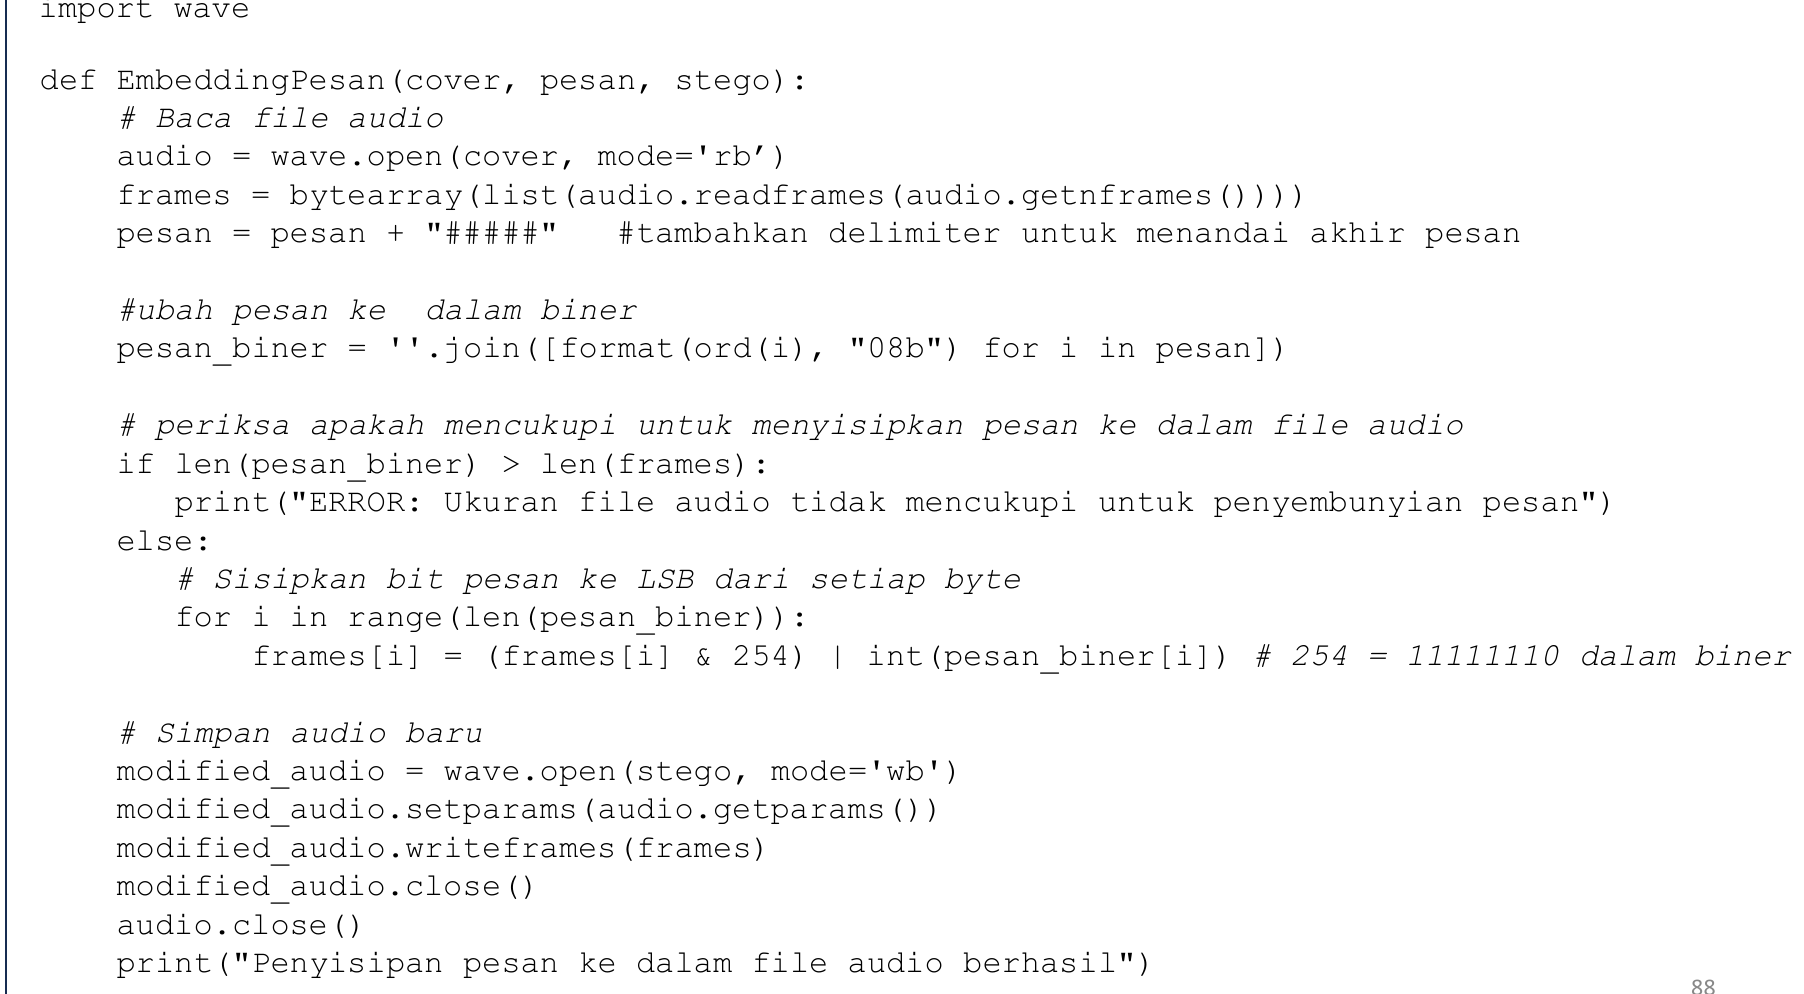
\includegraphics[width=197.40mm,height=273.24mm]{../../images/llm/page_088_img_01.png}%
\end{textblock*}

\end{document}
